\chapter{Introduction}
Lorem ipsum dolor sit amet, consectetuer adipiscing \textbf{Figure \ref{fig:model}} elit. Vivamus elementum sem eget tortor. Pellentesque id orci cursus sem tempus porttitor. Aenean tincidunt, neque vitae bibendum lacinia, magna erat dapibus nunc, vel pharetra nibh erat ac lorem. Ut suscipit ante eget magna. Morbi luctus aliquet odio. 

\section{Subsection}
Aenean turpis velit, ullamcorper sed, viverra vel, consectetuer sit amet, \cite{KunChen2005} Chenipsum. Phasellus sed lectus. Vivamus fermentum odio sed odio. Donec a dui. Duis et neque quis ligula pulvinar porttitor. Nunc mattis lectus vitae diam. 

Praesent quis orci. Aliquam id urna. Sed dolor erat, faucibus et, mattis eget, \textbf{commodo} nec, lorem. Etiam sit amet nisi sit amet nisi posuere bibendum. \emph{Cum sociis natoque} penatibus et magnis dis parturient montes, nascetur ridiculus mus. 


\begin{figure}
\centering
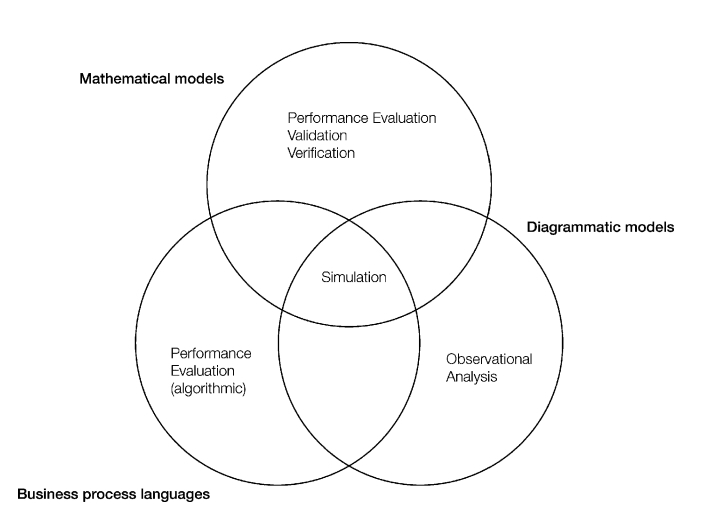
\includegraphics[scale=0.65]{./images/T1Figure01.pdf} 
\caption{caption text}
\label{fig:model}
\end{figure}

\begin{itemize}
\item Aliquam
\item mus
\item montes
\end{itemize}

\subsubsection{Subsubsection}
Lorem ipsum dolor sit amet, consectetuer adipiscing elit. Vivamus elementum sem eget tortor. Pellentesque id orci cursus sem tempus porttitor. Aenean tincidunt, neque vitae bibendum lacinia, magna erat dapibus \textbf{Table \ref{tab:table}} nunc, vel pharetra nibh erat ac lorem. Ut suscipit ante eget magna. Morbi luctus aliquet odio. Aenean turpis velit, ullamcorper sed, viverra vel, 

 \begin{table} [t] 
\centering
\begin{small}
\caption{Table caption text}
\label{tab:table}
\setlength{\tabcolsep}{1em}
\begin{tabular}{ l| p{8cm}}
\hline
 \textbf{X} & \textbf{ Y} \\
\hline
 \hline	
 Item1 & description\\
 \hline
  Item2 & description  \\
 \hline
  Item2 & description \\
 \hline
\end{tabular}
\end{small}
\end{table}



